% Created 2011-07-13 Wed 15:46
\documentclass[presentation]{beamer}
\usepackage[latin1]{inputenc}
\usepackage[T1]{fontenc}
\usepackage{fixltx2e}
\usepackage{graphicx}
\usepackage{longtable}
\usepackage{float}
\usepackage{wrapfig}
\usepackage{soul}
\usepackage{textcomp}
\usepackage{marvosym}
\usepackage{wasysym}
\usepackage{latexsym}
\usepackage{amssymb}
\usepackage{hyperref}
\tolerance=1000
\usepackage[english]{babel} \usepackage{ae,aecompl}
\usepackage{mathpazo,courier,euler} \usepackage[scaled=.95]{helvet}
\usepackage{listings}
\lstset{language=Python, basicstyle=\ttfamily\bfseries,
commentstyle=\color{red}\itshape, stringstyle=\color{darkgreen},
showstringspaces=false, keywordstyle=\color{blue}\bfseries}
\providecommand{\alert}[1]{\textbf{#1}}

\title{}
\author{FOSSEE}
\date{}

\usetheme{Warsaw}\usecolortheme{default}\useoutertheme{infolines}\setbeamercovered{transparent}
\begin{document}











\begin{frame}

\begin{center}
\vspace{12pt}
\textcolor{blue}{\huge Using python modules}
\end{center}
\vspace{18pt}
\begin{center}
\vspace{10pt}

\includegraphics[scale=0.95]{../images/fossee-logo.png}\\
\vspace{5pt}
\scriptsize Developed by FOSSEE Team, IIT-Bombay. \\ 
\scriptsize Funded by National Mission on Education through ICT\\
\scriptsize  MHRD,Govt. of India\\

\includegraphics[scale=0.30]{../images/iitb-logo.png}\\
\end{center}
\end{frame}
\begin{frame}
\frametitle{Objectives}
\label{sec-2}

  At the end of this tutorial, you will be able to ,


\begin{itemize}
\item Execute python scripts from command line.
\item Use import in scripts.
\item Import scipy and pylab modules.
\item Use python standard modules and 3rd party modules.
\end{itemize}
\end{frame}
\begin{frame}
\frametitle{Pre-requisite}
\label{sec-3}

Spoken tutorial on -

\begin{itemize}
\item Using plot interactively.
\item Embellishing a plot.
\item Saving plots.
\end{itemize}
\end{frame}
\begin{frame}[fragile]
\frametitle{Running Python script from command line}
\label{sec-4}


\begin{itemize}
\item Create a script, open text editor and type the following
\begin{verbatim}
     print "hello world!"
     print
\end{verbatim}

\item Save the script as \verb~hello.py~
\end{itemize}
\end{frame}
\begin{frame}[fragile]
\frametitle{Running Python script from command line (cont'd)}
\label{sec-5}


\begin{itemize}
\item Run the script
\begin{verbatim}
     $ python hello.py
\end{verbatim}

\end{itemize}
  \emph{Syntax :} \textbf{python filename}
\end{frame}
\begin{frame}
\frametitle{Four plot problem}
\label{sec-6}

    \begin{center}
      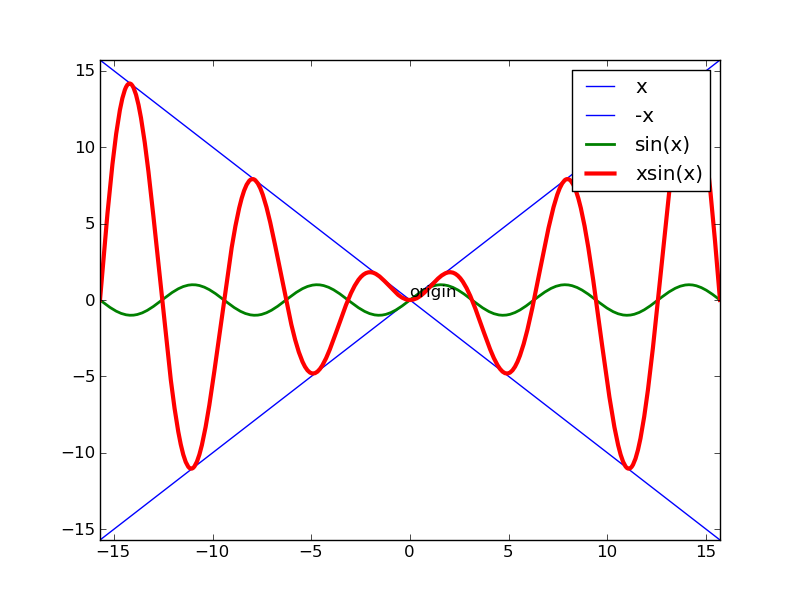
\includegraphics[scale=0.4]{four_plot}    
    \end{center}
\end{frame}
\begin{frame}[fragile]
\frametitle{Fix \verb~linspace()~ problem}
\label{sec-7}

\begin{verbatim}
   from scipy import *
\end{verbatim}
\end{frame}
\begin{frame}[fragile]
\frametitle{Fix \verb~plot()~ problem}
\label{sec-8}

\begin{verbatim}
   from pylab import *
\end{verbatim}
\end{frame}
\begin{frame}[fragile]
\frametitle{Better way of fixing}
\label{sec-9}

\begin{verbatim}
   from scipy import linspace
\end{verbatim}

  instead of
\begin{verbatim}
   from scipy import *
\end{verbatim}

    \verb~*~ means import all functions from name-space \verb~scipy~.
\end{frame}
\begin{frame}[fragile]
\frametitle{Instead of \verb~*~}
\label{sec-10}

\begin{verbatim}
    from scipy import linspace, pi, sin
    from pylab import plot, legend, annotate
    from pylab import xlim, ylim, title, show
\end{verbatim}

  Is better than, \verb~from scipy import *~ \& \verb~from pylab import *~.
\end{frame}
\begin{frame}[fragile]
\frametitle{Another Fix}
\label{sec-11}

\lstset{language=Python}
\begin{lstlisting}
import scipy
import pylab
x = scipy.linspace(-5*scipy.pi, 5*scipy.pi, 500)
pylab.plot(x, x, 'b')
pylab.plot(x, -x, 'b')
pylab.plot(x, scipy.sin(x), 'g', linewidth=2)
pylab.plot(x, x*scipy.sin(x), 'r', linewidth=3)
pylab.legend(['x', '-x', 'sin(x)', 'xsin(x)'])
pylab.annotate('origin', xy = (0, 0))
pylab.xlim(-5*scipy.pi, 5*scipy.pi)
pylab.ylim(-5*scipy.pi, 5*scipy.pi)
\end{lstlisting}
\end{frame}
\begin{frame}
\frametitle{Exercise 1}
\label{sec-12}


\begin{itemize}
\item Write a python script to plot a sine wave from 
    $-2\Pi$
  to 
    $2\Pi$
  .
\end{itemize}
\end{frame}
\begin{frame}
\frametitle{What is a module?}
\label{sec-13}

  Module is simply a file containing Python definitions and
  statements. Definitions from a module can be imported into other
  modules or into the main module.
\end{frame}
\begin{frame}
\frametitle{Python standard library}
\label{sec-14}

  Python has a very rich standard library of modules.

\begin{itemize}
\item Few libraries
\begin{itemize}
\item Math: \verb~math~, \verb~random~
\item Internet access: \verb~urllib2~, \verb~smtplib~
\item System, Command line arguments: \verb~sys~
\item Operating system interface: \verb~os~
\item regular expressions: \verb~re~
\item compression: \verb~gzip~, \verb~zipfile~, \verb~tarfile~
\end{itemize}
\item More information
\begin{itemize}
\item \href{http://docs.python.org/library}{http://docs.python.org/library}
\end{itemize}
\end{itemize}
\end{frame}
\begin{frame}
\frametitle{Summary}
\label{sec-15}

  In this tutorial, we have learnt to,


\begin{itemize}
\item Run scripts from command line,
\item Import modules by specifying the module name followed by  
    an asterisk.
\item Import only the required functions from modules by specifying 
    the function name.
\item Use python standard library.
\end{itemize}
\end{frame}
\begin{frame}
\frametitle{Evaluation}
\label{sec-16}


\begin{enumerate}
\item Which among this is correct ?
\begin{itemize}
\item from scipy import plot
\item from numpy import plot
\item from matplotlib import plot
\item from pylab import plot
\end{itemize}
\vspace{2pt}
\item Which among these libraries is part of python standard library ?
\begin{itemize}
\item Mayavi
\item scipy
\item matplotlib
\item urllib2
\end{itemize}
\vspace{2pt}
\item Functions ``xlim()'' and ``ylim()'' can be imported to the current
   name-space as,
\begin{itemize}
\item from pylab import xlim, ylim
\item import pylab
\item from scipy import xlim, ylim
\item import scipy
\end{itemize}
\end{enumerate}
\end{frame}
\begin{frame}
\frametitle{Solutions}
\label{sec-17}


\begin{enumerate}
\item from pylab import plot
\vspace{12pt}
\item urllib2
\vspace{12pt}
\item from pylab import xlim, ylim
\end{enumerate}
\end{frame}
\begin{frame}

 \begin{block}{}
  \begin{center}
  \textcolor{blue}{\Large THANK YOU!} 
  \end{center}
  \end{block}
\begin{block}{}
  \begin{center}
    For more Information, visit our website\\
    \url{http://fossee.in/}
  \end{center}  
  \end{block}
\end{frame}

\end{document}